\chapter{Additional information to Chapter~\ref{chapter:2023-sym-and-herpesvirus}}
\label{appendix:2023-sym-and-herpesvirus}

%%%%%%%%%%%%%%%%%%%%%%%%%%%%%%%%%%%%%%%%%%%%%%%%%%%%%%%%%%%%%%%%%%%%%%%%
%%%%%%%%%%%%%%%%%%%%%%%%%%%%%%%%%%%%%%%%%%%%%%%%%%%%%%%%%%%%%%%%%%%%%%%%
\section{Supplementary tables}


\begin{table}[h]
    \centering
    \caption[Description of the 59 (yes--no) symptoms available in the data and domain]{Description of the 59 (yes--no) symptoms available in the data and domain. Symptoms marked with an asterisk were removed due to a percentage of missing values higher than 25\%.}
    % \resizebox{0.8\linewidth}{!}{\begin{tabular}{lll}
% {p{0.2\textwidth} p{0.5\textwidth} {\centering}p{0.3\textwidth}}
% {m{0.2\textwidth} m{0.5\textwidth} m{0.3\textwidth}}
\toprule
Symptom & Description & Domain \\ 
\midrule
% Autonomic
airhunger           & Air hunger, difficulty breathing, or shortness of breath on exertion/activity & Autonomic \\
bladderprob         & Bladder problems & Autonomic \\
dizzystandup        & Dizzyness while standing up & Autonomic \\
extremepale         & Being extremely pale & Autonomic \\
ibssymptoms         & IBS symptoms & Autonomic \\
intolstandup        & Intolerance to standing up & Autonomic \\
lightheaded         & Feeling lightheaded & Autonomic \\
palpitations\textsuperscript{${\ast}$}    & Palpitations & Autonomic \\
palpitstandup       & Palpitations while standing up & Autonomic \\
sick\_nausea\textsuperscript{${\ast}$}    & Feeling sick/nausea & Autonomic \\
% Immunological
alcoholintoler\textsuperscript{${\ast}$}  & Intolerance to alcohol & Immunological \\
feverchills         & Fever/Chills & Immunological \\
fewviralinfect\textsuperscript{${\ast}$}  & Fewer viral infections than before & Immunological \\
flusymptoms         & Flu symptoms & Immunological \\
freqviralinfect     & Frequent viral infections with long recovery periods & Immunological \\
newsensit           & Worsen sensitivity to light & Immunological \\
sorethroat          & Sore throat & Immunological \\
stiffnessmorn       & Morning stiffness & Immunological \\
tenderglands        & Tender glands & Immunological \\
% Neuroendocrine
coldhandsfeet\textsuperscript{${\ast}$} & Unusual cold hands or feet & Neuroendocrine \\
intolheat\_cold   & Intolerance to extremes of heat/cold & Neuroendocrine \\
sexualfunction    & Decreased sexual function or interest & Neuroendocrine \\
unusualsweaty     & Unusually sweaty & Neuroendocrine \\
weightchange\textsuperscript{${\ast}$}  & Abnormal appetite or change in weight & Neuroendocrine \\
worsepoststress   & Worsening of symptoms post stress & Neuroendocrine \\
% Neurocognitive
backweak        & Back weakness & Neurocognitive \\
brainfog        & Brain fog or confusion & Neurocognitive \\
concentprob     & Trouble concentrating & Neurocognitive \\
diffdecisions\textsuperscript{${\ast}$}  & Difficulty making decisions & Neurocognitive \\
diffretaininfo  & Difficulty retaining or recalling info & Neurocognitive \\
diffunderstand  & Difficulty understanding things/thinking clearly & Neurocognitive \\
diffwords\textsuperscript{${\ast}$}   & Difficulty finding or saying word & Neurocognitive \\
disorientation  & Disorientation & Neurocognitive \\
eyesightdistub  & Eyesight disturbance (temporary) & Neurocognitive \\
lossbalance     & Loss of balance or unsteadiness while standing, unable to focus the vision & Neurocognitive \\
muscdisc        & Muscle discomfort & Neurocognitive \\
muscweak        & Muscle weakness & Neurocognitive \\
neckweak        & Neck weakness & Neurocognitive \\
poorcoord       & Poor coordination or unsteady movements (while walking) & Neurocognitive \\
senstlightnoise & Sensitivity to light/noise & Neurocognitive \\
shortmem        & Short term memory problems & Neurocognitive \\
slowthink       & Slow thinking & Neurocognitive \\
tingling        & Tingling/numbness in arms and/or legs & Neurocognitive \\
twitching\textsuperscript{${\ast}$}   & Muscle twitching & Neurocognitive \\
% Pain
chestabdpain     & Pain in chest or abdomen & Pain \\
diffmigraine     & Migraine which is different/worse than before & Pain \\
jointpain\textsuperscript{${\ast}$}    & Pain in two or more joints w/o infamm. & Pain \\
jointpainnoinnfl & Joint pain w/o inflamm. & Pain \\
muscpain         & Muscle pain & Pain \\
newheadache      & Headaches which are new/worse than before & Pain \\
% Post-exertional malaise
exerciseintol       & Intolerance to exercise & Post-exertional malaise \\
fatiguediffaterill  & Fatigue/exhaustion after activity that would not cause fatigue before & Post-exertional malaise \\
fatiguelast24h\textsuperscript{${\ast}$}  & Fatigue/exhaustion after effort, lasting >24h & Post-exertional malaise \\
malaise24h          & Malaise after exertion, lasting >24h & Post-exertional malaise \\
markedfatigexertion & Marked physical/mental fatigue/exhaustion after minimal effort, lasting >24h & Post-exertional malaise \\
painexertion        & Pain after exertion/effort, lasting >24h & Post-exertional malaise \\
worsesympmore24h    & Worsening of symptoms after exertion/effort, lasting >24h & Post-exertional malaise \\
% Sleep
sleepproblems   & Problems in sleep, quality of duration; insomnia & Sleep \\
unrefsleep      & Unrefreshing sleep & Sleep \\
\bottomrule
\end{tabular}}
    \resizebox{\linewidth}{!}{\begin{tabular}{lll}
% {p{0.2\textwidth} p{0.5\textwidth} {\centering}p{0.3\textwidth}}
% {m{0.2\textwidth} m{0.5\textwidth} m{0.3\textwidth}}
\toprule
Symptom & Description & Domain \\ 
\midrule
% Autonomic
airhunger           & Air hunger, difficulty breathing, or shortness of breath on exertion/activity & Autonomic \\
bladderprob         & Bladder problems & Autonomic \\
dizzystandup        & Dizzyness while standing up & Autonomic \\
extremepale         & Being extremely pale & Autonomic \\
ibssymptoms         & IBS symptoms & Autonomic \\
intolstandup        & Intolerance to standing up & Autonomic \\
lightheaded         & Feeling lightheaded & Autonomic \\
palpitations\textsuperscript{${\ast}$}    & Palpitations & Autonomic \\
palpitstandup       & Palpitations while standing up & Autonomic \\
sick\_nausea\textsuperscript{${\ast}$}    & Feeling sick/nausea & Autonomic \\
% Immunological
alcoholintoler\textsuperscript{${\ast}$}  & Intolerance to alcohol & Immunological \\
feverchills         & Fever/Chills & Immunological \\
fewviralinfect\textsuperscript{${\ast}$}  & Fewer viral infections than before & Immunological \\
flusymptoms         & Flu symptoms & Immunological \\
freqviralinfect     & Frequent viral infections with long recovery periods & Immunological \\
newsensit           & Worsen sensitivity to light & Immunological \\
sorethroat          & Sore throat & Immunological \\
stiffnessmorn       & Morning stiffness & Immunological \\
tenderglands        & Tender glands & Immunological \\
% Neuroendocrine
coldhandsfeet\textsuperscript{${\ast}$} & Unusual cold hands or feet & Neuroendocrine \\
intolheat\_cold   & Intolerance to extremes of heat/cold & Neuroendocrine \\
sexualfunction    & Decreased sexual function or interest & Neuroendocrine \\
unusualsweaty     & Unusually sweaty & Neuroendocrine \\
weightchange\textsuperscript{${\ast}$}  & Abnormal appetite or change in weight & Neuroendocrine \\
worsepoststress   & Worsening of symptoms post stress & Neuroendocrine \\
% Neurocognitive
backweak        & Back weakness & Neurocognitive \\
brainfog        & Brain fog or confusion & Neurocognitive \\
concentprob     & Trouble concentrating & Neurocognitive \\
diffdecisions\textsuperscript{${\ast}$}  & Difficulty making decisions & Neurocognitive \\
diffretaininfo  & Difficulty retaining or recalling info & Neurocognitive \\
diffunderstand  & Difficulty understanding things/thinking clearly & Neurocognitive \\
diffwords\textsuperscript{${\ast}$}   & Difficulty finding or saying word & Neurocognitive \\
disorientation  & Disorientation & Neurocognitive \\
eyesightdistub  & Eyesight disturbance (temporary) & Neurocognitive \\
lossbalance     & Loss of balance or unsteadiness while standing, unable to focus the vision & Neurocognitive \\
muscdisc        & Muscle discomfort & Neurocognitive \\
muscweak        & Muscle weakness & Neurocognitive \\
neckweak        & Neck weakness & Neurocognitive \\
poorcoord       & Poor coordination or unsteady movements (while walking) & Neurocognitive \\
senstlightnoise & Sensitivity to light/noise & Neurocognitive \\
shortmem        & Short term memory problems & Neurocognitive \\
slowthink       & Slow thinking & Neurocognitive \\
tingling        & Tingling/numbness in arms and/or legs & Neurocognitive \\
twitching\textsuperscript{${\ast}$}   & Muscle twitching & Neurocognitive \\
% Pain
chestabdpain     & Pain in chest or abdomen & Pain \\
diffmigraine     & Migraine which is different/worse than before & Pain \\
jointpain\textsuperscript{${\ast}$}    & Pain in two or more joints w/o infamm. & Pain \\
jointpainnoinnfl & Joint pain w/o inflamm. & Pain \\
muscpain         & Muscle pain & Pain \\
newheadache      & Headaches which are new/worse than before & Pain \\
% Post-exertional malaise
exerciseintol       & Intolerance to exercise & Post-exertional malaise \\
fatiguediffaterill  & Fatigue/exhaustion after activity that would not cause fatigue before & Post-exertional malaise \\
fatiguelast24h\textsuperscript{${\ast}$}  & Fatigue/exhaustion after effort, lasting >24h & Post-exertional malaise \\
malaise24h          & Malaise after exertion, lasting >24h & Post-exertional malaise \\
markedfatigexertion & Marked physical/mental fatigue/exhaustion after minimal effort, lasting >24h & Post-exertional malaise \\
painexertion        & Pain after exertion/effort, lasting >24h & Post-exertional malaise \\
worsesympmore24h    & Worsening of symptoms after exertion/effort, lasting >24h & Post-exertional malaise \\
% Sleep
sleepproblems   & Problems in sleep, quality of duration; insomnia & Sleep \\
unrefsleep      & Unrefreshing sleep & Sleep \\
\bottomrule
\end{tabular}}
    \label{appendix:taba1-sym-bin-description}
\end{table}
% Supplementary Table 1
% Supplementary Table~\ref{appendix:taba1-sym-bin-description}

\begin{table}[h]
    \centering
    \caption[Percentage of individuals with presence of each symptom, across multiple sclerosis, ME/CFS as a single cohort, and ME/CFS separated into four distinct subgroups]{Percentage of individuals with presence of each symptom, across multiple sclerosis (MS), ME/CFS as a single cohort, and ME/CFS separated into four distinct subgroups. Symptoms marked with an asterisk were removed due to a high percentage of missing values and percentages were not estimated. Differences in sample sizes from Table~\ref{tab:tab1-basic-characteristics-cfs-ms} reflect the removal of some individuals due to a large proportion of missing data across the symptoms.}
    \resizebox{0.6\linewidth}{!}{\begin{tblr}{
    row{1} = {m},
    column{1} = {l},
    column{2-7} = {c},
    hline{1,61} = {-}{0.08em},
    hline{2} = {-}{0.05em},
}
Symptom code & {MS\\($n=39$)} & {ME/CFS\\($n=222$)} & {ME/CFS\_S0\\($n=41$)} & {ME/CFS\_S1\\($n=43$)} & {ME/CFS\_S2\\($n=92$)} & {ME/CFS\_S3\\($n=46$)}\\
airhunger           & 25.64 & 58.48 & 60.98 & 41.86 & 63.04 & 62.50\\
bladderprob         & 71.79 & 56.70 & 56.10 & 44.19 & 59.78 & 62.50\\
dizzystandup        & 17.95 & 68.30 & 65.85 & 58.14 & 73.91 & 68.75\\
extremepale         & 10.26 & 49.55 & 43.90 & 41.86 & 47.83 & 64.58\\
ibssymptoms         & 38.46 & 78.12 & 82.93 & 72.09 & 76.09 & 83.33\\
intolstandup        & 41.03 & 51.79 & 43.90 & 37.21 & 61.96 & 52.08\\
lightheaded         & 30.77 & 73.21 & 68.29 & 65.12 & 78.26 & 75.00\\
palpitations\textsuperscript{${\ast}$}    & --- & --- & --- & --- & --- & ---\\
palpitstandup       & 5.13 & 33.93 & 26.83 & 32.56 & 39.13 & 31.25\\
sick\_nausea\textsuperscript{${\ast}$}    & --- & --- & --- & --- & --- & ---\\
alcoholintoler\textsuperscript{${\ast}$}  & --- & --- & --- & --- & --- & ---\\
feverchills & 7.69  & 57.59 & 60.98 & 39.53 & 65.22 & 56.25\\
fewviralinfect\textsuperscript{${\ast}$}  & --- & --- & --- & --- & --- & ---\\
flusymptoms         & 10.26 & 71.88 & 73.17 & 53.49 & 78.26 & 75.00\\
freqviralinfect     & 5.13 & 52.68 & 56.10 & 32.56 & 57.61 & 58.33\\
newsensit           & 15.38 & 66.07 & 56.10 & 62.79 & 68.48 & 72.92\\
sorethroat          & 7.69 & 71.88 & 65.85 & 60.47 & 77.17 & 77.08\\
stiffnessmorn       & 66.67 & 70.98 & 65.85 & 72.09 & 70.65 & 75.00\\
tenderglands        & 12.82 & 75.45 & 75.61 & 58.14 & 81.52 & 79.17\\
coldhandsfeet\textsuperscript{${\ast}$}   & --- & --- & --- & --- & --- & ---\\
intolheat\_cold     & 58.97 & 74.55 & 80.49 & 69.77 & 73.91 & 75.00\\
sexualfunction      & 58.97 & 57.14 & 56.10 & 58.14 & 60.87 & 50.00\\
unusualsweaty       & 7.69 & 55.36 & 51.22 & 51.16 & 55.43 & 62.50\\
weightchange\textsuperscript{${\ast}$}    & --- & --- & --- & --- & --- & ---\\
worsepoststress     & 71.79 & 89.29 & 85.37 & 86.05 & 90.22 & 93.75\\
backweak            & 30.77 & 62.95 & 65.85 & 62.79 & 59.78 & 66.67\\
brainfog            & 53.85 & 77.23 & 70.73 & 72.09 & 83.70 & 75.00\\
concentprob         & 61.54 & 95.98 & 90.24 & 97.67 & 96.74 & 97.92\\
diffdecisions\textsuperscript{${\ast}$}   & --- & --- & --- & --- & --- & ---\\
diffretaininfo      & 53.85 & 81.70 & 70.73 & 81.40 & 89.13 & 77.08\\
diffunderstand      & 46.15 & 82.59 & 73.17 & 81.40 & 89.13 & 79.17\\
diffwords\textsuperscript{${\ast}$}       & --- & --- & --- & --- & --- & ---\\
disorientation      & 25.64 & 50.45 & 48.78 & 34.88 & 58.70 & 50.00\\
eyesightdistub      & 66.67 & 60.71 & 60.98 & 48.84 & 64.13 & 64.58\\
lossbalance         & 89.74 & 73.66 & 73.17 & 67.44 & 79.35 & 68.75\\
muscdisc            & 48.72 & 86.16 & 87.80 & 83.72 & 85.87 & 87.50\\
muscweak            & 66.67 & 85.27 & 90.24 & 72.09 & 86.96 & 89.58\\
neckweak            & 25.64 & 54.91 & 53.66 & 55.81 & 53.26 & 58.33\\
poorcoord           & 71.79 & 62.05 & 58.54 & 55.81 & 66.30 & 62.50\\
senstlightnoise     & 30.77 & 77.68 & 65.85 & 65.12 & 89.13 & 77.08\\
shortmem            & 61.54 & 83.48 & 80.49 & 74.42 & 90.22 & 81.25\\
slowthink           & 41.03 & 75.89 & 65.85 & 60.47 & 84.78 & 81.25\\
tingling            & 82.05 & 69.64 & 68.29 & 62.79 & 67.39 & 81.25\\
twitching\textsuperscript{${\ast}$}       & --- & --- & --- & --- & --- & ---\\
chestabdpain        & 35.90 & 77.23 & 78.05 & 81.40 & 75.00 & 77.08\\
diffmigraine        & 10.26 & 38.39 & 31.71 & 39.53 & 39.13 & 41.67\\
jointpain\textsuperscript{${\ast}$}       & --- & --- & --- & --- & --- & ---\\
jointpainnoinnfl    & 20.51 & 55.36 & 51.22 & 53.49 & 56.52 & 58.33\\
muscpain            & 51.28 & 87.95 & 90.24 & 86.05 & 86.96 & 89.58\\
newheadache         & 28.21 & 77.23 & 75.61 & 79.07 & 77.17 & 77.08\\
exerciseintol       & 41.03 & 81.70 & 75.61 & 72.09 & 84.78 & 89.58\\
fatiguediffaterill  & 71.79 & 96.43 & 90.24 & 100.00 & 96.74 & 97.92\\
fatiguelast24h\textsuperscript{${\ast}$}  & --- & --- & --- & --- & --- & ---\\
malaise24h          & 30.77 & 95.98 & 92.68 & 90.70 & 97.83 & 100.00\\
markedfatigexertion & 33.33 & 77.68 & 73.17 & 69.77 & 82.61 & 79.17\\
painexertion        & 25.64 & 75.89 & 70.73 & 72.09 & 75.00 & 85.42\\
worsesympmore24h    & 30.77 & 91.07 & 85.37 & 88.37 & 94.57 & 91.67\\
sleepproblems       & 51.28 & 85.71 & 78.05 & 81.40 & 90.22 & 87.50\\
unrefsleep          & 61.54 & 98.66 & 100.00 & 100.00 & 97.83 & 97.92\\
\end{tblr}}
    \label{appendix:taba2-percentage-sym-bin}
\end{table}
% Supplementary Table 2
% Supplementary Table~\ref{appendix:taba2-percentage-sym-bin}


\begin{table}[h]
    \centering
    \caption[AUC and its 95\% confidence interval, optimal cutoff and associated sensitivity and specificity to discriminate patients with multiple sclerosis from healthy controls]{AUC and its 95\% confidence interval (CI), optimal cutoff and associated sensitivity (Se) and specificity (Sp) to discriminate patients with multiple sclerosis (cases) from healthy controls. In the Direction column, the symbols ``{>}'' and ``{<}'' represent higher value in MS cases than in healthy controls and vice-versa, respectively. In the Cutoff column, the p-value within brackets came from the Pearson’s $\chi^2$ test with Yates' correction for $2 \times 2$ tables after being adjusted for a false discovery rate of 5\% using the Benjamini-Hochberg procedure. In the AUC column, the symbol ``{$\ast$}'' denote the cases where there is evidence of AUC different from 0.50 (random guess).}
    \resizebox{\linewidth}{!}{\begin{tabular}{lccccc}
\toprule
Herpesvirus & Direction & AUC (95\% CI) & Cutoff (p-value) & Se & Sp \\
\midrule
CMV         & $\text{controls}>\text{cases}$ & 0.513 (0.398, 0.629) & 196.84 (0.0155) & 0.9000 & 0.000 \\
EBV-EBNA1   & $\text{controls}<\text{cases}$ & 0.584 (0.488, 0.680) & 20.515 (0.0073) & 0.950 & 0.306 \\
EBV-VCA     & $\text{controls}<\text{cases}$ & 0.641 (0.538, 0.744) & 139.235 (0.0073) & 0.650 & 0.643 \\
HHV6        & $\text{controls}<\text{cases}$ & 0.539 (0.427, 0.650) & 148.91 (0.0799) & 0.125 & 0.969 \\
HSV1        & $\text{controls}>\text{cases}$ & 0.626 (0.531, 0.721)\textsuperscript{${\ast}$} & 3.72 (0.0073) & 0.950 & 0.327 \\
HSV2        & $\text{controls}<\text{cases}$ & 0.544 (0.437, 0.650) & 6.875 (0.0799) & 0.550 & 0.633 \\
VZV         & $\text{controls}>\text{cases}$ & 0.573 (0.461, 0.685) & 172.575 (0.0595) & 0.425 & 0.765 \\
\bottomrule
\end{tabular}
% \begin{tblr}{
%     row{1} = {m},
%     column{1} = {l},
%     column{2-5} = {c},
%     hline{1,9} = {-}{0.08em},
%     hline{2} = {-}{0.05em},
% }
% Herpesvirus & Direction & AUC (95\% CI) & Cutoff (p-value) & Se & Sp \\
% CMV         & $\text{controls}>\text{cases}$ & 0.513 (0.398, 0.629) & 196.84 (0.0155) & 0.9000 & 0.000 \\
% EBV-EBNA1   & $\text{controls}<\text{cases}$ & 0.584 (0.488, 0.680) & 20.515 (0.0073) & 0.950 & 0.306 \\
% EBV-VCA     & $\text{controls}<\text{cases}$ & 0.641 (0.538, 0.744) & 139.235 (0.0073) & 0.650 & 0.643 \\
% HHV6        & $\text{controls}<\text{cases}$ & 0.539 (0.427, 0.650) & 148.91 (0.0799) & 0.125 & 0.969 \\
% HSV1        & $\text{controls}>\text{cases}$ & 0.626 (0.531, 0.721)\textsuperscript{${\ast}$} & 3.72 (0.0073) & 0.950 & 0.327 \\
% HSV2        & $\text{controls}<\text{cases}$ & 0.544 (0.437, 0.650) & 6.875 (0.0799) & 0.550 & 0.633 \\
% VZV         & $\text{controls}>\text{cases}$ & 0.573 (0.461, 0.685) & 172.575 (0.0595) & 0.425 & 0.765 \\
% \end{tblr}}
    \label{appendix:taba3-models-auc-optimal-cutoff-ms}
\end{table}
% Supplementary Table 3
% Supplementary Table~\ref{appendix:taba3-models-auc-optimal-cutoff-ms}

\clearpage
%%%%%%%%%%%%%%%%%%%%%%%%%%%%%%%%%%%%%%%%%%%%%%%%%%%%%%%%%%%%%%%%%%%%%%%%
%%%%%%%%%%%%%%%%%%%%%%%%%%%%%%%%%%%%%%%%%%%%%%%%%%%%%%%%%%%%%%%%%%%%%%%%
\section{Supplementary figures}


\begin{figure}[h]
    \centering
    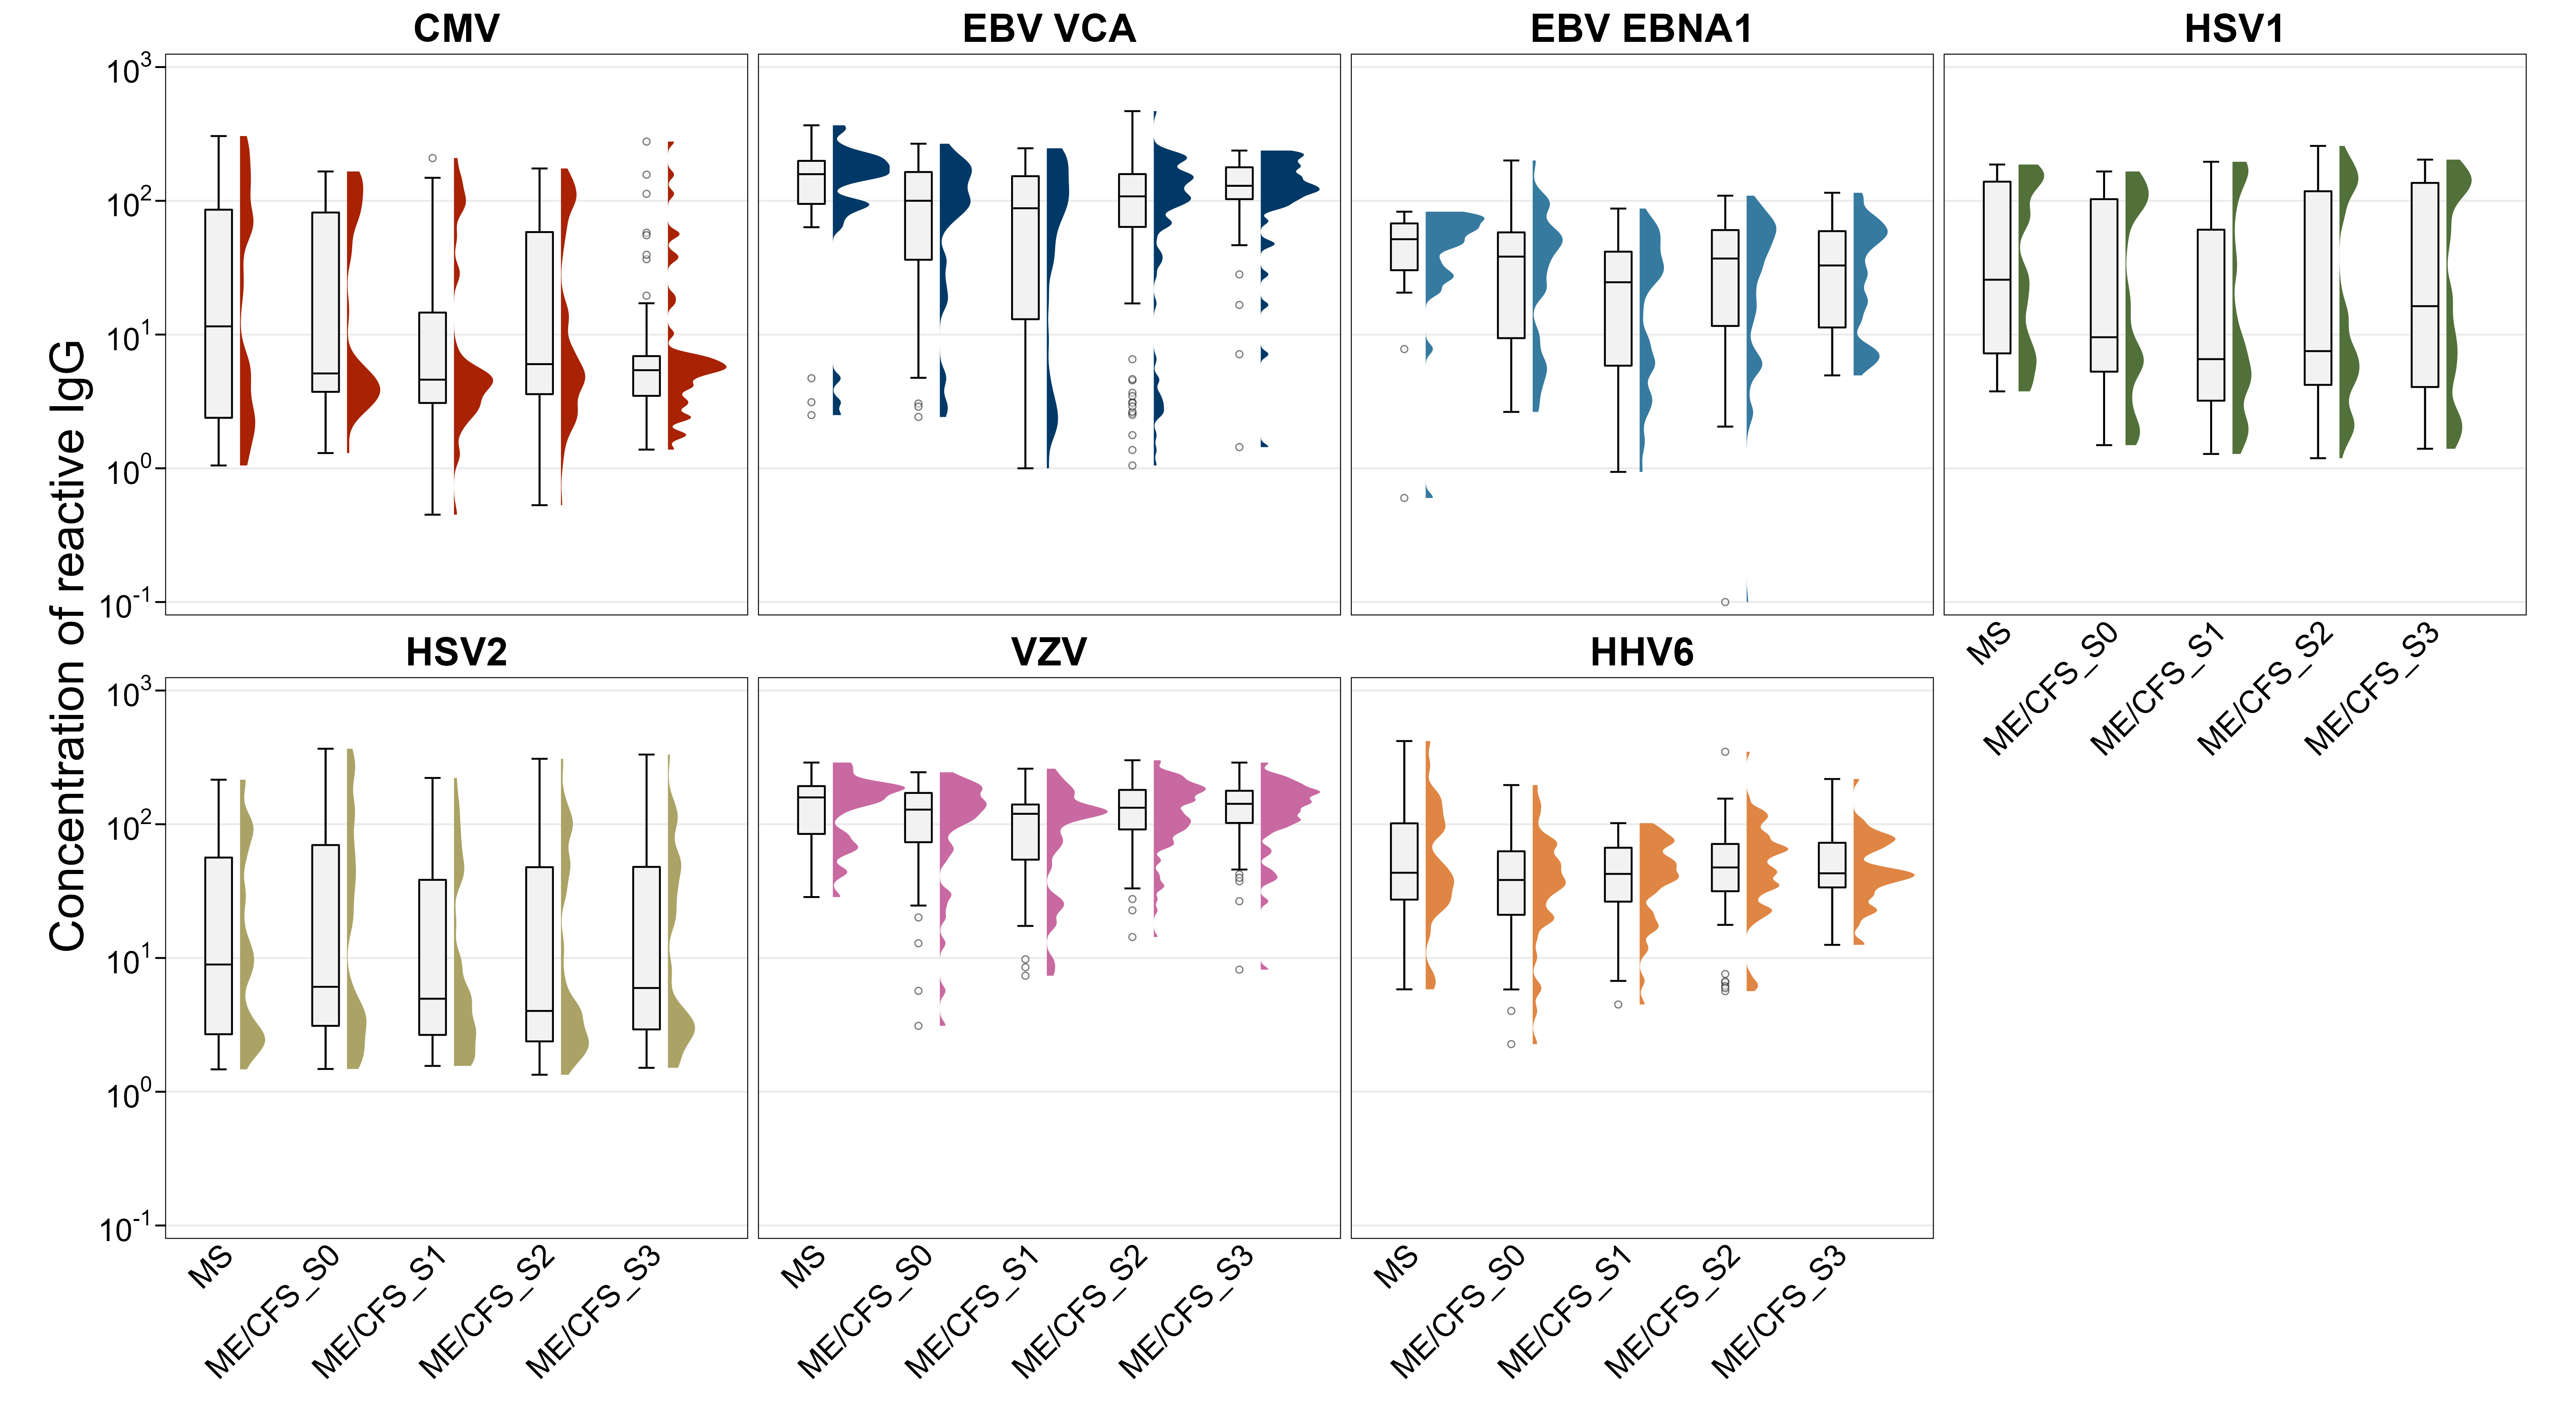
\includegraphics[width=0.95\textwidth]{chapter/2023-sym-and-herpesvirus/figures/figa1-quantitative-serology.png}
    \caption[Quantitative serology data per study group and herpesvirus/antigen]{Quantitative serology data per study group and herpesvirus/antigen.}
    \label{appendix:figa1-quantitative-serology}
\end{figure}
% Supplementary Figure 1
% Supplementary Figure~\ref{appendix:figa1-quantitative-serology}


\begin{figure}[h]
    \centering
    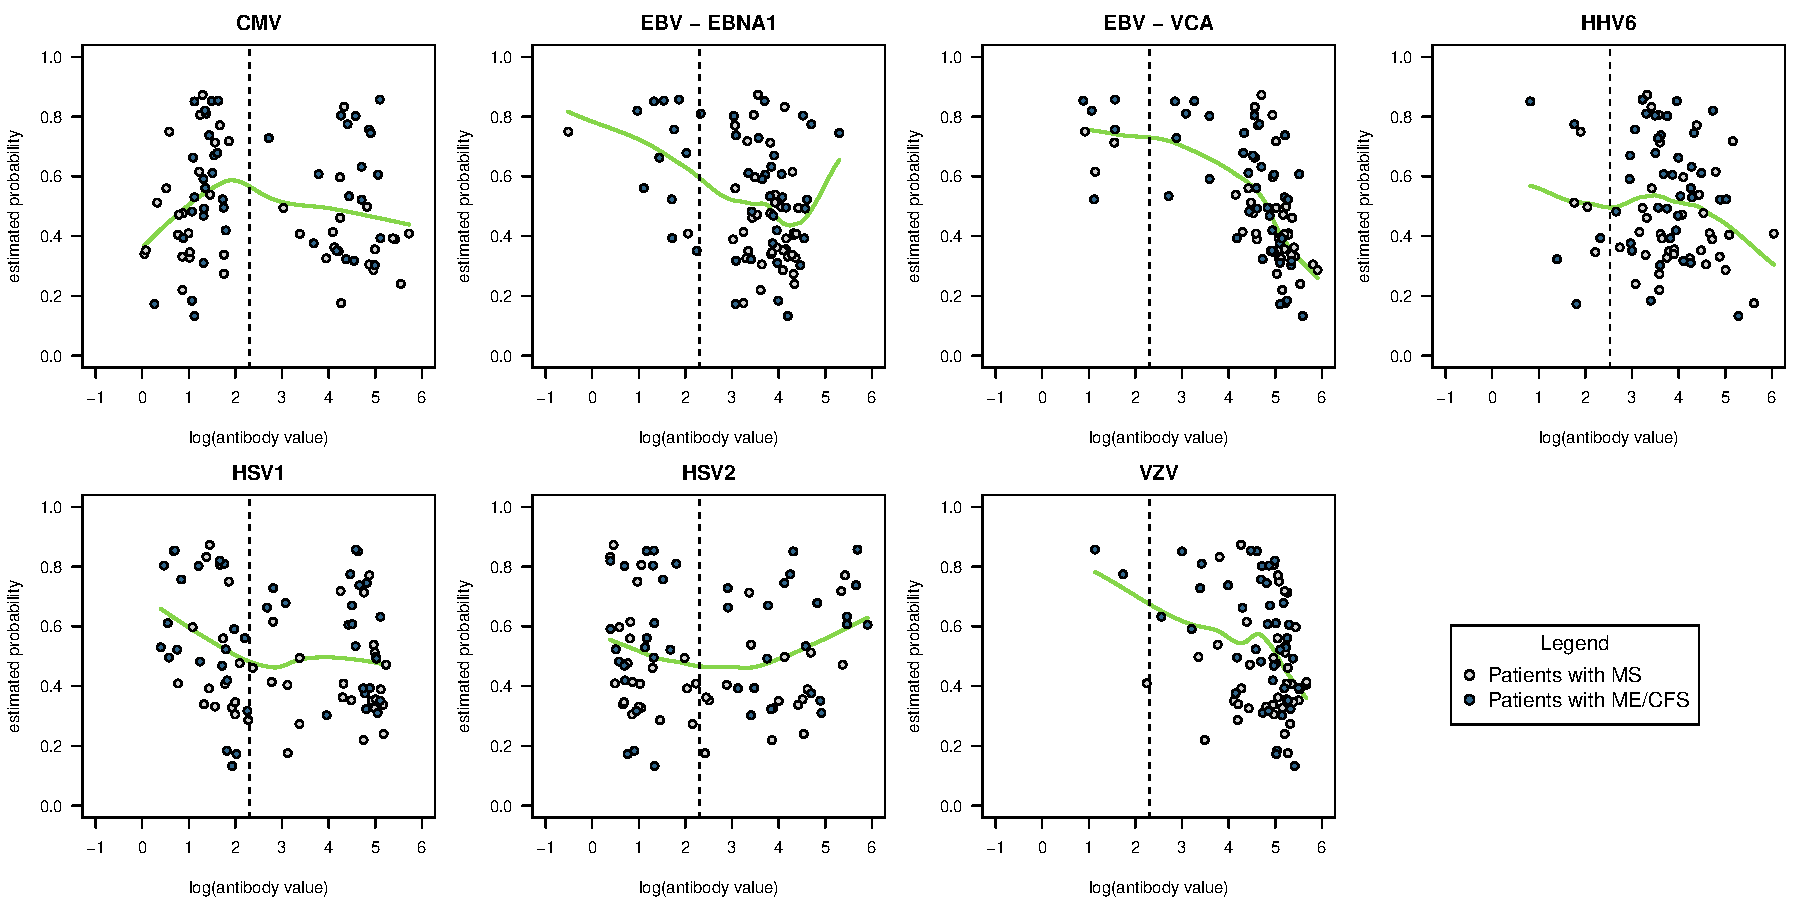
\includegraphics[width=0.95\textwidth]{chapter/2023-sym-and-herpesvirus/figures/figa2-ms-vs-s0.pdf}
    \caption[Smooth-line approximations of the relationship between log(antibody values) and SL-estimated probability of ME/CFS\_S0 patient when compared to patients with MS.]{Smooth-line approximations (green lines) of the relationship between log(antibody values) and SL-estimated probability of ME/CFS\_S0 patient when compared to patients with MS. Each dot represents a patient and the vertical dashed lines represent the cut-off for seropositivity according to the respective lab protocol.}
    \label{appendix:figa2-ms-vs-s0}
\end{figure}
% Supplementary Figure 2
% Supplementary Figure~\ref{appendix:figa2-ms-vs-s0}


\begin{figure}[h]
    \centering
    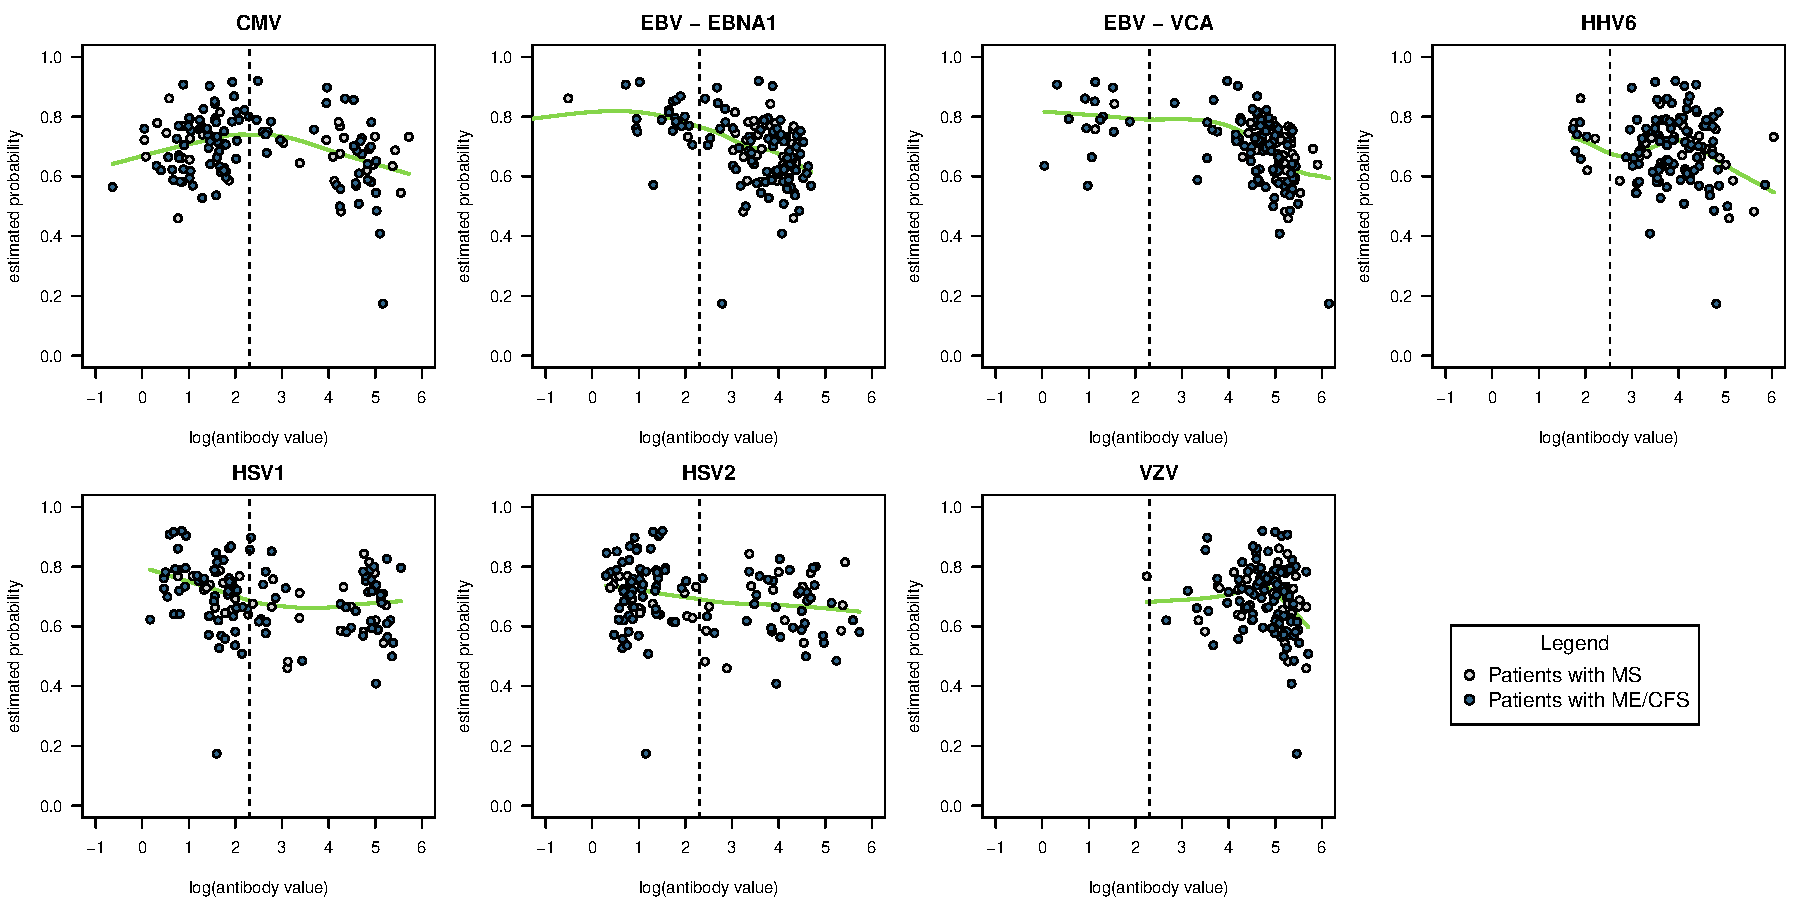
\includegraphics[width=0.95\textwidth]{chapter/2023-sym-and-herpesvirus/figures/figa3-ms-vs-s2.pdf}
    \caption[Smooth-line approximations of the relationship between log(antibody values) and SL-estimated probability of ME/CFS\_S2 patient when compared to patients with MS.]{Smooth-line approximations (green lines) of the relationship between log(antibody values) and SL-estimated probability of ME/CFS\_S2 patient when compared to patients with MS. Each dot represents a patient and the vertical dashed lines represent the cut-off for seropositivity according to the respective lab protocol.}
    \label{appendix:figa3-ms-vs-s2}
\end{figure}
% Supplementary Figure 3
% Supplementary Figure~\ref{appendix:figa3-ms-vs-s2}


\begin{figure}[h]
    \centering
    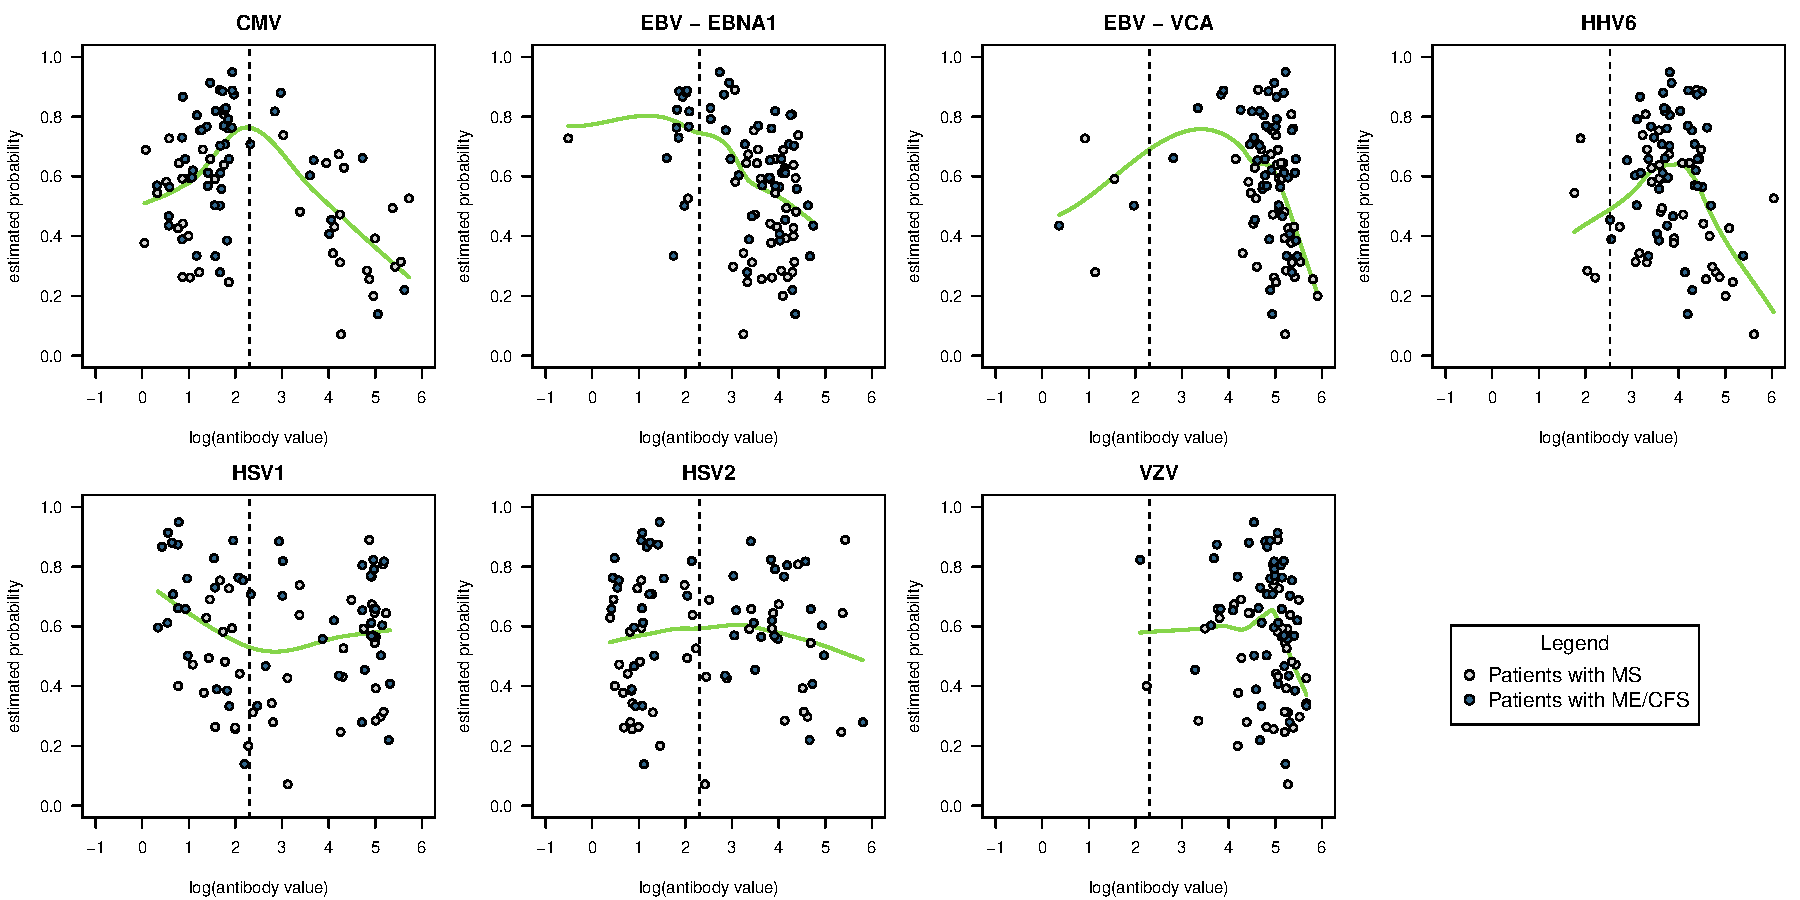
\includegraphics[width=0.95\textwidth]{chapter/2023-sym-and-herpesvirus/figures/figa4-ms-vs-s3.pdf}
    \caption[Smooth-line approximations of the relationship between log(antibody values) and SL-estimated probability of ME/CFS\_S3 patient when compared to patients with MS.]{Smooth-line approximations (green lines) of the relationship between log(antibody values) and SL-estimated probability of ME/CFS\_S3 patient when compared to patients with MS. Each dot represents a patient and the vertical dashed lines represent the cut-off for seropositivity according to the respective lab protocol.}
    \label{appendix:figa4-ms-vs-s3}
\end{figure}
% Supplementary Figure 4
% Supplementary Figure~\ref{appendix:figa4-ms-vs-s3}